\documentclass[conference]{IEEEtran}
\usepackage{graphicx}
\usepackage{algorithm}
\usepackage{algorithmic}

\makeatletter
\def\BState{\State\hskip-\ALG@thistlm}
\makeatother



\begin{document}
\title{Write an efficient algorithm to merge two given large Heaps of different sizes to create one large Heap. Do this merging using Heap Insertion approach where you insert elements of one Heap, one-by-one, into the other Heap. Trace the movement of elements in every step of the execution of your algorithm. }

\author{\IEEEauthorblockN{Parag Parihar}
\IEEEauthorblockA{Roll No:- IIT2016095\\
iit2016095@iiita.ac.in}
\and
\IEEEauthorblockN{Rakshit Sai}
\IEEEauthorblockA{Roll No:- IIT2016126\\
iit2016126@iiita.ac.in}
\and
\IEEEauthorblockN{Adarsh Agrawal}
\IEEEauthorblockA{Roll No:- IIT2016516\\
iit2016516@iiita.ac.in}
\and
\IEEEauthorblockN{Nilotpal Pramanik}
\IEEEauthorblockA{Roll No:- IRM2016501\\
irm2016501@iiita.ac.in}
\thanks{Manuscript received February 2, 2018.}}

\markboth{Assignment-1, IDAA432C; B.Tech.(IT)}
{Shell \MakeLowercase{\textit{et al.}}: Bare Demo of IEEEtran.cls for Journals}

\maketitle

\IEEEpeerreviewmaketitle

\section{\textbf{Introduction and Literature Survey}}

The question is basically on heaps. The heap data structure is generally taught with the heap sort. The most common use of heaps is when we want to access the largest or the smallest item. It is one of the widely used data structure.If you think Heap as a binary tree sorted in linear order by depth with the root node first; then the children of a node at index N are 2N+1 and 2N+2. So the most basic usage of heaps is in picking up the maximum and minimum elements.

Now coming to the given problem we had to write an efficient algorithm in-order to merge two large heaps of given sizes to create a single large Heap. We have to merge these two heaps using the insertion approach where we insert the elements of one heap one by one into the other heap. Finally we need to keep record of the movement of every step when we move the elements from one Heap to another Heap. The above problem allows us to compare two heaps side by side and see how each of their index behaves when the elements are removed one by one from one heap and put into the other one by applying concepts of array of linked lists. This shows that how heaps allow us to deal with multiple maximums and minimums at a time. This can be extended to larger number of Heaps also.

\section{\textbf{Algorithm Design}}
According to the problem we have to write an efficient algorithm to merge two given large Heaps of different sizes to create one large Heap. Do this merging using Heap Insertion approach where we have to insert elements of one Heap, one-by-one, into the other Heap. Trace the movement of elements in every step of the execution of the algorithm.\\

First of all we are taking the input, the length of the two large heaps respectively through “n”,”m” as well as two large heaps “heap1” and “heap2”.We have to find the comparatively longer heap and scan that heap first and after that we will scan the other heap in to $index\_arr$,a defined array of length 2000000 has been used for storing the elements of the two different heaps accordingly.And we will call the “merge” function taking the lengths of the heaps as the attributes.\\

In the “merge” function firstly, we are storing $InsertAtEnd(track[index\_arr[i]], i)$ in $track[index\_arr[i]]$, track is an already defined structure “struct” of “node” having length 2000000.Struct node only contains an integer “data” and the struct of node “next” itself.\\
As well as we will assign “i” at the index.And again through for loop we will run for the length of the another heap and in $heap1[index]$ we will $store\ heap2[j]$ as well as $InsertAtEnd(track[index\_arr[index]], index)$ will be stored in $track[index\_arr[index]]$.\\

While for till non zero i and satisfying $heap1[parent(i)]<heap1[i]$ condition we will now store the $InsertAtEnd(track[index\_arr[parent(i)]], i)$ in the head  track$[index\_arr[parent(i)]]$ and $InsertAtEnd(track[index\_arr[i]], parent(i))$ in the head  $track[index\_arr[i]]$.Then swap between the $index\ i$ and	$parent(i)$ using swap function after that we will  assign the value of $parent(i)$ at i.\\

In the above mentioned “parent” function we are taking the index “i” as the attribute and returning only the $(i-1)/2$ value.\\

After running the while loop we have to increment the value of index by one and assign the index at i.Then we will print the “after insertion of the element of heap2(smaller one) i.e j+1 itself.After that we will print the track and heap1 by calling the print function through running for loops upto the total length of the heaps respectively.\\

In the print function we are taking the struct node* head as the attribute and in the function assign the head at temp, a struct node type variable.And till temp not equal to null we will print its corresponding data and reassign the next address to the temp.\\

Above mentioned function “InsertAtEnd” have the return type struct node* and taking the struct node* next and the index as the attributes.In the function assign the head at temp, a struct node type variable using malloc for dynamic allocation.Then in $temp \rightarrow data$ we will assign the value of “x”.Then we have to check whether the value of head is null or not.If true then we will assign the value of head at $temp \rightarrow next$, temp to head and return the value of head.Otherwise we will assign the value of head at $temp1 \rightarrow next$ , an another instance of struct node.Then check the condition for nullity and follow the same three steps to return the value of head.\\

\begin{algorithm}[H]
\caption{InsertAtEnd function}
\end{algorithm}
\begin{algorithmic}[1]
\STATE \textbf{INPUT: \textit{head, x }}
\STATE \textbf{OUTPUT: \textit{new node at end of linked list}}
\STATE \textbf{Initialization} : $ temp ,temp1(struct pointer)$ 
\STATE Allocate memory to temp
\STATE $(temp \rightarrow data) \gets x$
\IF{$head = NULL$}
	\STATE $(temp \rightarrow next) \gets head$
	\STATE $head \gets temp $
	\STATE \textbf{return} head
\ELSE
	\STATE $temp1 \gets head$
    \WHILE{ $temp1 \rightarrow next \neq NULL$}
    	\STATE $temp1 \gets (temp1 \rightarrow next)$
     \ENDWHILE   
        \STATE $(temp1 \rightarrow next) \gets temp$
        \STATE $(temp \rightarrow next) \gets NULL$
        \STATE \textbf{return} head
\ENDIF
\end{algorithmic}

\begin{algorithm}[H]
\caption{Swap function}
\end{algorithm}
\begin{algorithmic}[1]
\STATE \textbf{INPUT: \textit{ x,y }}
\STATE \textbf{Initialization} : $ temp$ 
\STATE $temp \gets heap1[x]$
\STATE $heap1[x] \gets heap1[y]$
\STATE $heap1[y] \gets  temp$
\STATE $temp \gets index\_arr[y]$
\STATE $index\_arr[y] \gets index\_arr[x]$
\STATE $index\_arr[x] \gets temp$
\end{algorithmic}

\begin{algorithm}[H]
\caption{Merge function}
\end{algorithm}
\begin{algorithmic}[1]
\STATE \textbf{INPUT: length of heap1(a), length of heap2(b)}
\STATE \textbf{Initialization} : i,j,k
\FOR{i 0 to a}
	\STATE $track[index\_arr[i]] \gets InsertAtEnd(track[index\_arr[i]], i)$
\ENDFOR
\STATE $ index \gets i$
\FOR{j 0 to b }
	\STATE $heap1[index] \gets heap2[j]$
    \STATE $track[index\_arr[index]] \gets InsertAtEnd(track[index\_arr[index]], index)$
    \WHILE{$i \neq 0$ AND $(heap1[parent(i)] < heap1[i])$}
    	\STATE $track[index\_arr[parent(i)]] \gets InsertAtEnd(track[index\_arr[parent(i)]], i)$
        \STATE $track[index\_arr[i]] \gets InsertAtEnd(track[index\_arr[i]], parent(i))$
        \STATE $swap(i,parent(i))$
        \STATE $i \gets parent(i)$
    \ENDWHILE
    \STATE $index \gets index+1$;
    \STATE $i \gets index$
    \STATE Print the movement of each of the elements which were initially at ${k}_{th}$ index in heap1 after insertion of  ${j+1}_{th}$ element of heap2(smaller one).
    \STATE We use the linked list of the ${k}_{th}$ index of heap1(bigger one) for tracing.
\ENDFOR
\STATE print the merged heap having n+m elements.
\end{algorithmic}

\begin{algorithm}[H]
\caption{Main function}
\end{algorithm}
\begin{algorithmic}[1]
\STATE \textbf{Initialization} : $ i$
\STATE \textbf{\textbf{Scan} length of heaps (n,m)}
\IF{ $n > m$}
	\FOR{i 0 to n}
		\STATE \textbf{Scan} \ Heap1 AND update index\_arr[i] as i
    \ENDFOR
    \FOR{i 0 to m}
		\STATE \textbf{Scan} Heap2 AND update index\_arr[i+n] as i+n
    \ENDFOR
    \STATE \textbf{Call function:-} Merge(n,m)
\ELSE
	\FOR{i 0 to n}
		\STATE \textbf{Scan} Heap2 AND update index\_arr[i] as i
    \ENDFOR
    \FOR{i 0 to m}
		\STATE \textbf{Scan} Heap1 AND update index\_arr[i+n] as i+n
    \ENDFOR
    \STATE \textbf{Call function:-} Merge(m,n)
\ENDIF

\end{algorithmic}

   
\section{\textbf{Analysis and Discussion}}
\textbf{Linked List} : 1. if first node : 10 instructions \\
2. if not the the first node : 14 + 4m instructions\\
\textbf{Printing Function} : $3 + 4(m)$ instructions\\
\textbf{Swap function} : 15 instructions\\
\textbf{Printing in total} : $3 + 11m + 14m^2 + 8m^3$ instructions (depends strongly on execution, not of importance) = C1\\
\textbf{Parent Function} : 4 instructions\\ 
\textbf{Inserting an element in heap} : $(log_{2}n)$ instructions\\
\textbf{Merge Function} : $2n + 3 + 6n + 2m + m(14 + log_2(69 + 8m) + C1)$ instructions\\
\subsection{\textbf{Best Case}} : 	
The algorithm will have its best case when the largest element of smaller heap is less than the last element of the bigger heap, in this case the algorithm will not go in the while loop (running $log_2n$ times) hence it will execute in linear time.
Best Case proportional to,
		$11 + 21n + 38m + C2$  which is  $O(n + m)$.
        
\subsection{\textbf{Worst Case}} : 
Since to Inserting an element in heap takes (log2n) instructions, so we this can maximize when both n and m are equal, then only it will for maximum time.
	Worst Case proportional to,
		$11 + 52m + m(log_{2}(69 + 8m) + C1)  + C1$ which is  $O(nlog_{2}n)$

\subsection{\textbf{Average Case}} : 
We will have random cases with both cases not equal,hence all the cases will lie between worst and best, more towards $O(nlog_{2}n)$. 

\subsection{\textbf{Graph for Sum of Heap size vs Number of Iterations(Time Complexity)}} :\\
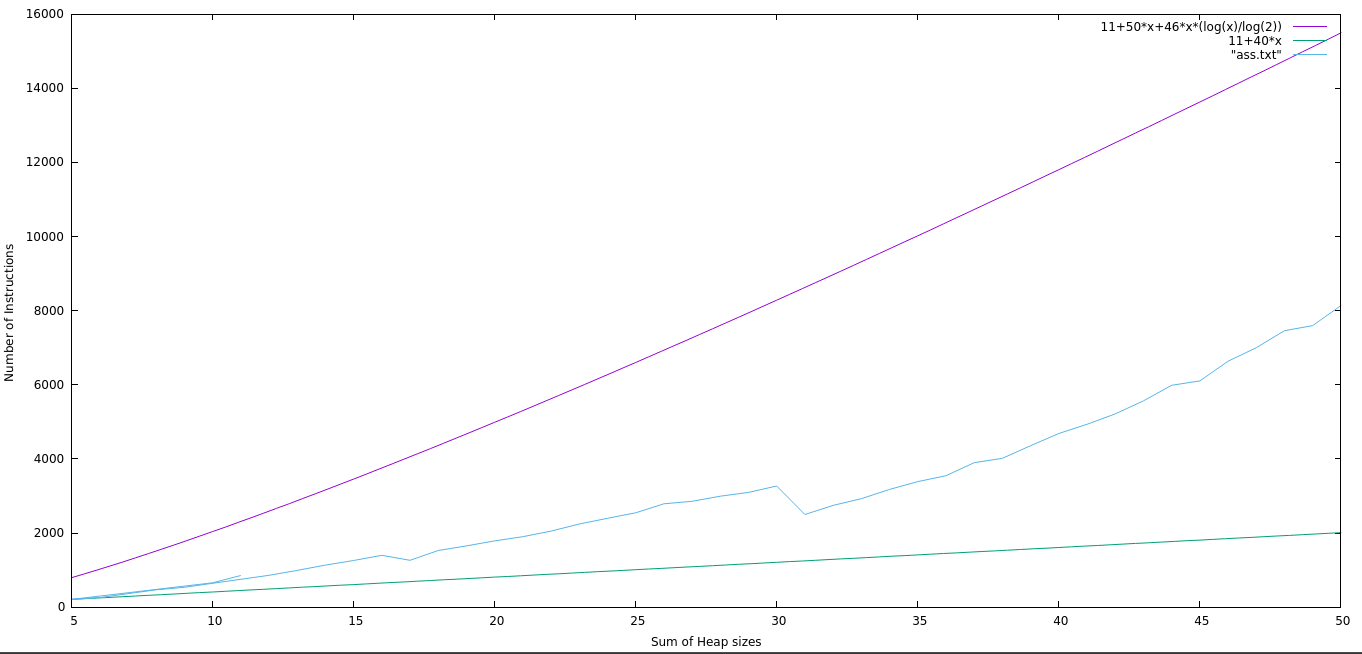
\includegraphics[height =  5.0cm,width = \linewidth]{time__1_.png}
First Curve : Worst Case.\\
Second Curve : Average Case.\\
Third Curve : Best Case.

\section{\textbf{Discussion}}
\textbf{Use of linked lists for storing movements}:-\\
As we were required to trace the movements of the elements at each step we insert a new element to the heap, since this can become really complicated in the arrays, we defined an array of linked lists to solve the problem, each index points to the next index that element moved from the current position.\\
We were swapping parents and children constantly, and everytime we added the next index in both of their separate linked lists, so as to keep the track of every element.\\

\textbf{Reducing time complexity}:-\\
We reduced the time complexity by checking, at the beginning, that which of the heaps is bigger, the one that is smaller will be the one from which we will remove elements and add into the larger one.For eg.
N = 16, M = 8\\
$16(log_28) > 8(log_216)$ ,i.e, $16*3 > 8*4$ ,i.e, $48 > 32$
And this difference will be much bigger for bigger values of n and m, hence checking at the start saves us from that problem.So, we reduced the complexity to,\\
	$$O(smaller(log_2(bigger))$$

\section{\textbf{Experimental Analysis}}
We revised the commands and basic functions of \textbf{GNUPlot} to plot the time complexity analysis graphs and other relevant analysis related to our algorithm.\\
While making this report we also learnt the basics of making reports using \textbf{LATEX} in \textbf{IEEE }format using \textbf{IEEEtran class}.\\\\
\     To find the time complexity graph, for given values of sizes of heap 1 and heap 2, we randomly generated their heap elements[using rand() \% 10], max heapify them to make them heaps and then for various values tried to find out the best case complexity instructions, worst case instructions and average case instructions.\\

As we know that we will get the worst case when both heaps are of same size and all the elements of an heap are smaller from even the smallest element of other heap.\\

Also the best case will be when the smaller heap has all the elements smaller than bigger heap.\\
We thereby increment a counter on every instruction performed and therefore derive the following table,
\begin{table}[h!]
\begin{center}
    \label{tab:table1}
    \begin{tabular}{|c|c|c|c|c|} % <-- Alignments: 1st column left, 2nd middle and 3rd right, with vertical lines in between
    \hline
     \textbf{Size of} & \textbf{Size of} & \textbf{Best} & \textbf{Average} & \textbf{Worst}\\
     \textbf{HEAP1(n)} & \textbf{HEAP2(m)} & \textbf{CASE} & \textbf{CASE} & \textbf{CASE}\\
      \hline
      07 & 01 & 216 & 231 & 261\\
      \hline
      03 & 03 & 297 & 327 & 357\\
      \hline
      04 & 04 & 470 & 515 & 545\\
      \hline
      05 & 05 & 659 & 749 & 764\\
      \hline
	  08 & 04 & 690 & 720 & 810\\
      \hline
	  06 & 06 & 861 & 966 & 981\\
      \hline
	  07 & 07 & 1075 & 1150 & 1225\\
      \hline
      08 & 08 & 1298 & 1403 & 1478\\
      \hline
      09 & 09 & 1529 & 1559 & 1724\\
      \hline
      50 & 50 & 14109 & 14709 & 15384\\
      \hline
      100 & 100 & 32794 & 34159 & 35404\\
      \hline
      1000 & 1000 & 480471 & 498561 & 507876\\
      \hline
    \end{tabular}
\end{center}
\end{table}
From the above table it is clear that in the best case we are getting $O(n + m)$ complexity but the worst being slightly greater is proportional to $O(nlog_2n)$, we are getting slight deviations because of the additional complexities because linked list and print functions(not of importance).



\section{\textbf{Conclusion}}

By making the proper analysis of the algorithm and optimizing the code as much as possible we can conclude that the best case algorithm will occur when the largest element of the smaller heap is smaller than the smallest element of the larger heap and the time complexity for it will be linear which is  Ω(n+m) where n and m are the size of the heaps. Now coming to the worst case of the algorithm the situation must be as such so that the implementation of the while loop always occur and the time complexity for the worst case of the algorithm is $O(nlog_{2}n)$. The average case lies in between these two and it is more inclined towards the worst case. Thus, by implementing the code designed for the given algorithm we have developed a optimized mechanism to merge two heaps into one. This way we can deal with many number of heaps by extending the above problem for n heaps.

\end{document}